% Chapter Template

\chapter{Results} % Main chapter title

\label{Chapter3} % Change X to a consecutive number; for referencing this chapter elsewhere, use \ref{ChapterX}

%-------------------------------------------------------------------------------------
%	SECTION 1
%-------------------------------------------------------------------------------------
\section{Definition of Error}
To assess the degree to which changes in the analysis pipeline affect the quality of measurement, a definition of error must first be decided upon. Error ($\epsilon$) is defined to be a function over pharynx space ($p$) which is the difference between the intensity measured in one frame and another. The difference is normalized by the average intensity of the two frames at 410 nm.


\[\epsilon(p) = \frac{I_{410_1}(p) - I_{410_2}(p)}{\frac{I_{410_1}(p) + I_{410_2}(p)}{2}}\]

To calculate redox potentials, we take the first frame at 410 nm and the second at 470 nm. When we quantify error, however, we must use a single wavelength as the changes in emission spectra would confound the errors.

%-------------------------------------------------------------------------------------
%	SECTION 2
%-------------------------------------------------------------------------------------
\section{Collection of test data} \label{testCollection}

A large number of technical replicates were collected. A single animal was plated on 5.5 mM levamisole and imaged 57 times in pairs of two images both at 410 nm. A paired-sample t-test indicates no significant difference (p=0.41) between the first and second intensity profile.

\begin{figure}[ht]
    \centering
    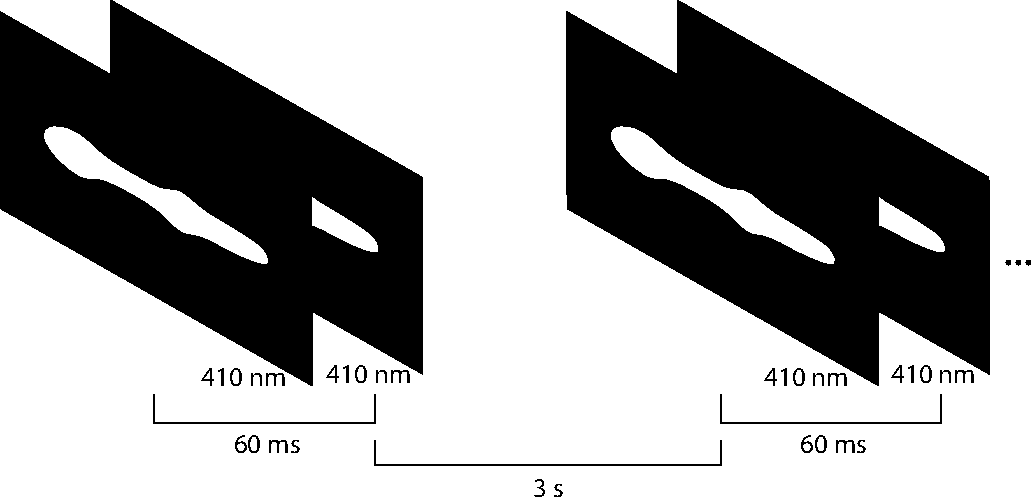
\includegraphics[scale=0.5]{Figures/rendered_files/test_imaging_schematic}
    \decoRule
    \caption[Test imaging schematic]{}
    \label{fig:TestImagingSchematic}
\end{figure}

%-------------------------------------------------------------------------------------
%	SECTION 3
%-------------------------------------------------------------------------------------
\section{A partially synthetic data set increases statistical power}

Instead of comparing pairs of measurements taken back-to-back, we can compare all possible pairs. Given n images, we generate ${n \choose 2} = \frac{n!}{2!(n-2)!}$ pairs. Repeated excitation seems to attenuate the emission amplitude of the sensor (Figure \ref{fig:AvgIntensityOverTime}). To account for this effect (known as photobleaching) we generate pairs starting at the 15th imaged pair, and excluding outliers (Figure \ref{fig:AvgIntensityOverTime}).

Since the average time between frames in this synthetic data set is 10 seconds\todo{do this calculation}, there is a large degree of inter-frame movement. Because the true test data has only 12 \todo{real number} pairs which display inter-frame movement, this partially synthetic data set allows us to be more confident about the changes in error seen using different analysis strategies.

\begin{figure}[ht]
    \centering
    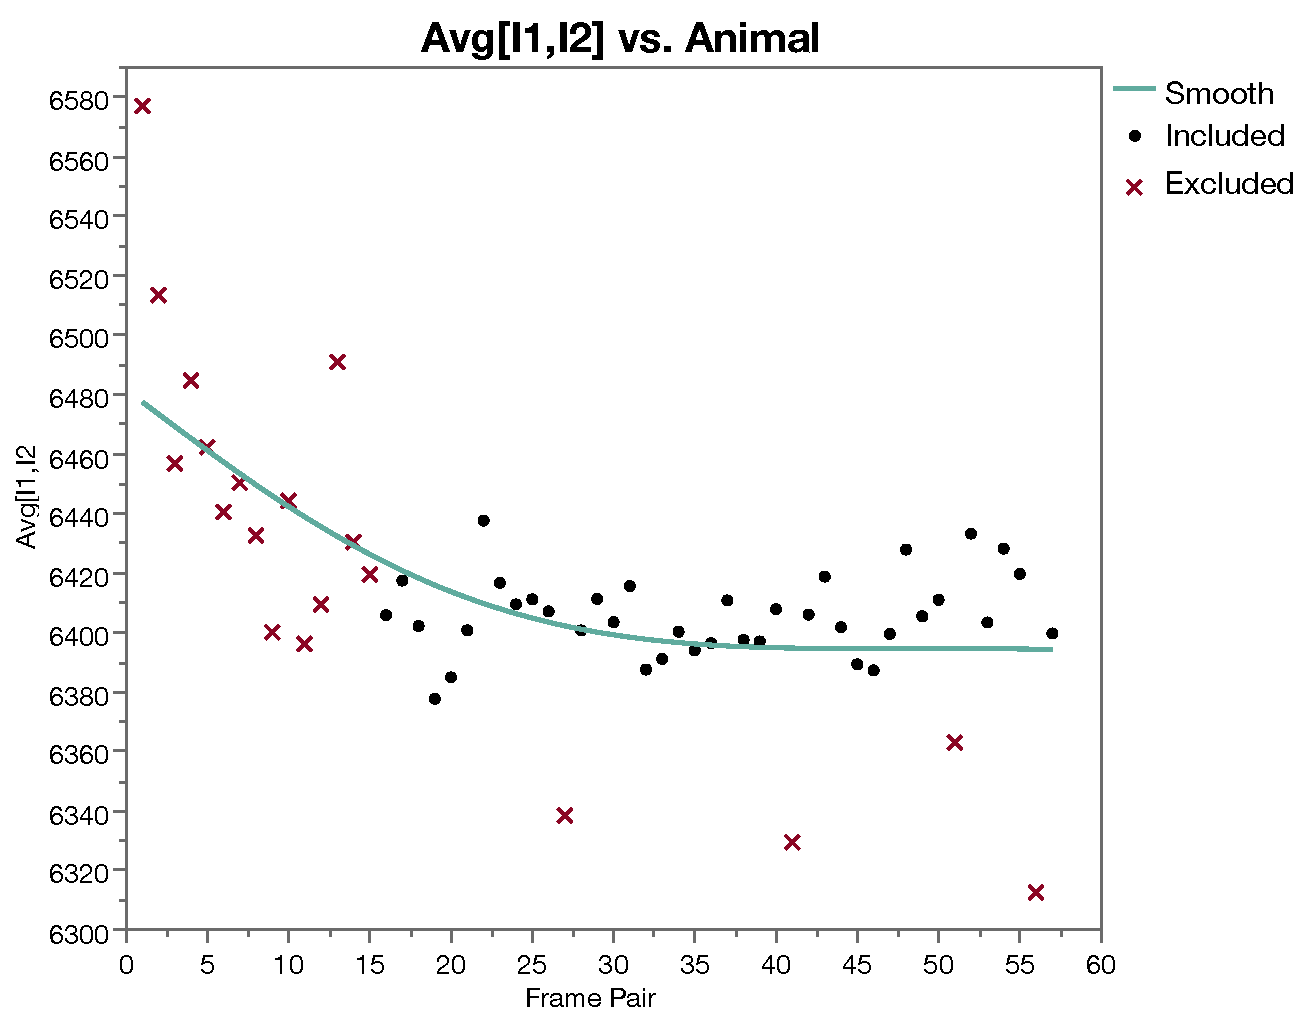
\includegraphics[scale=0.35]{Figures/rendered_files/photobleaching}
    \decoRule
    \caption[Average intensity over time in technical replicates]{The average intensity over time in technical replicates. Red xs mark image pairs excluded from the recombination.}
    \label{fig:AvgIntensityOverTime}
\end{figure}

%-------------------------------------------------------------------------------------
%	SECTION 4
%-------------------------------------------------------------------------------------
\section{Reductions in Manual Intervention}

\todo[inline]{show figures comparing \% requiring manual intervention for segmentation and for midlines}

%-------------------------------------------------------------------------------------
%	SECTION 5
%-------------------------------------------------------------------------------------
\section{Channel-Specific Masks and Midlines Reduce Error}

% \begin{figure}[ht]
%     \centering
%     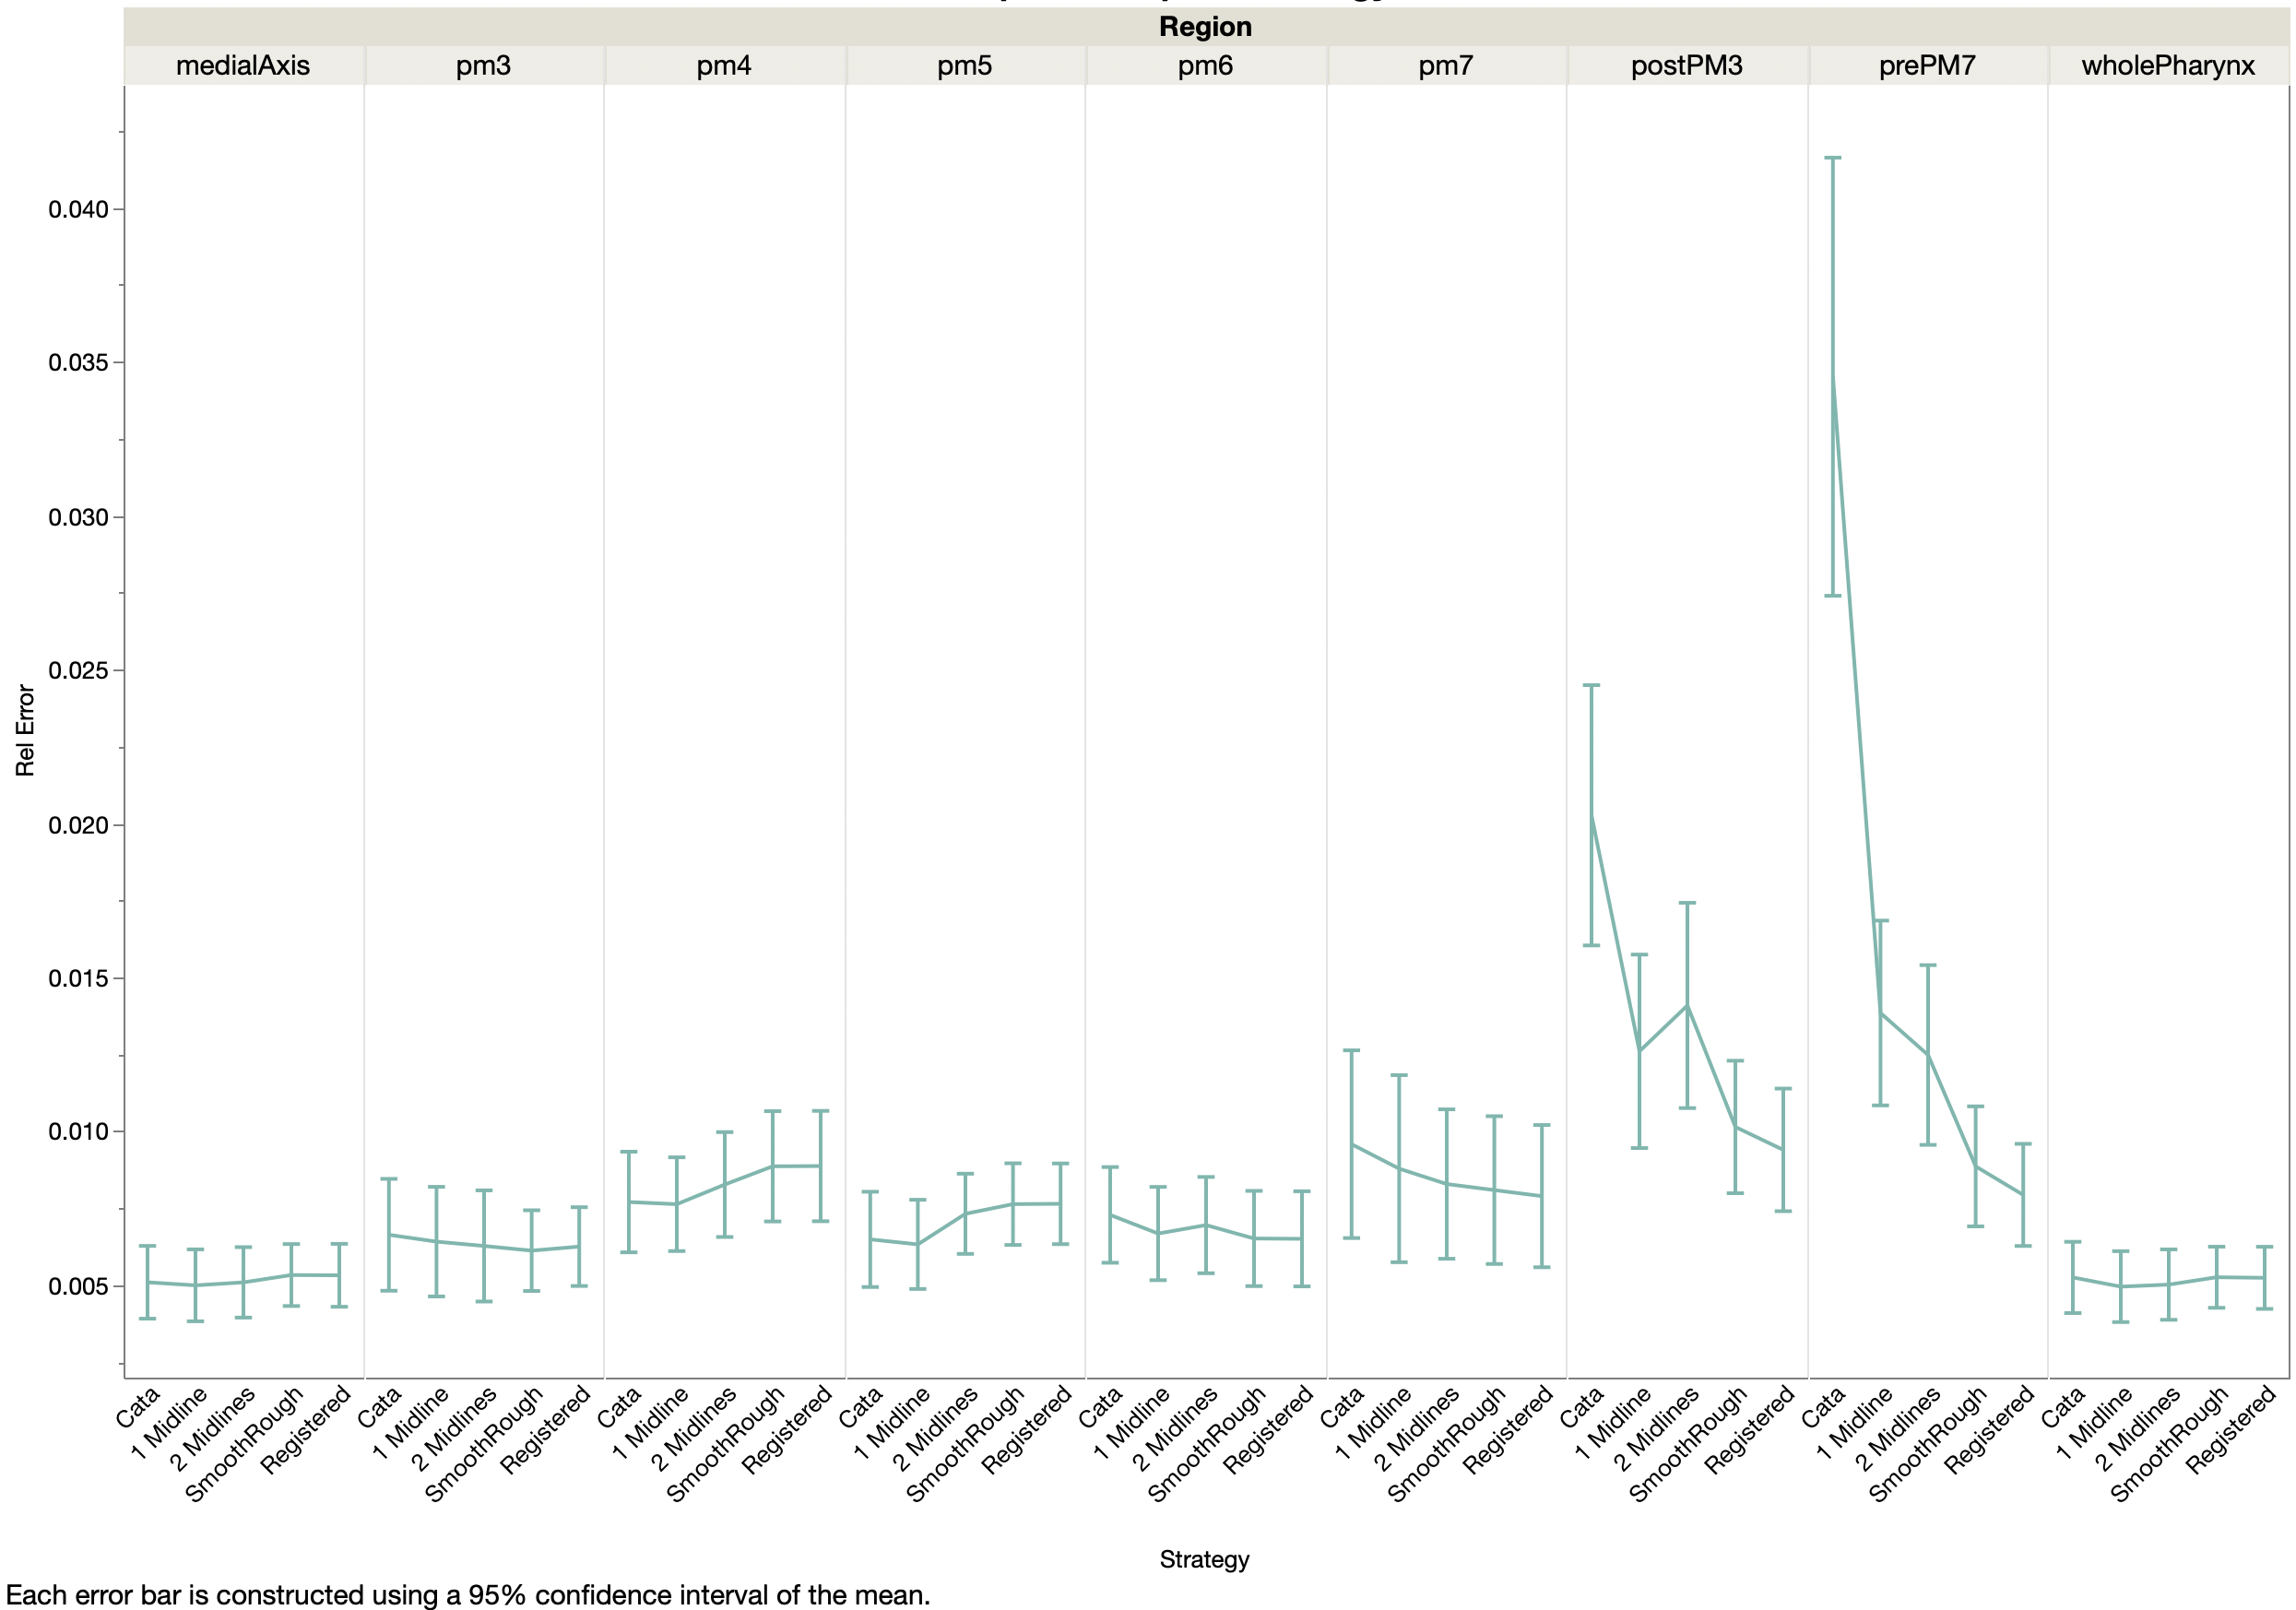
\includegraphics[scale=0.15]{Figures/rendered_files/error_by_strategy_natural}
%     \decoRule
%     \caption[Error by strategy in the natural data set]{Relative error}
%     \label{fig:PercentErrorNatural}
% \end{figure}

% \begin{figure}[ht]
%     \centering
%     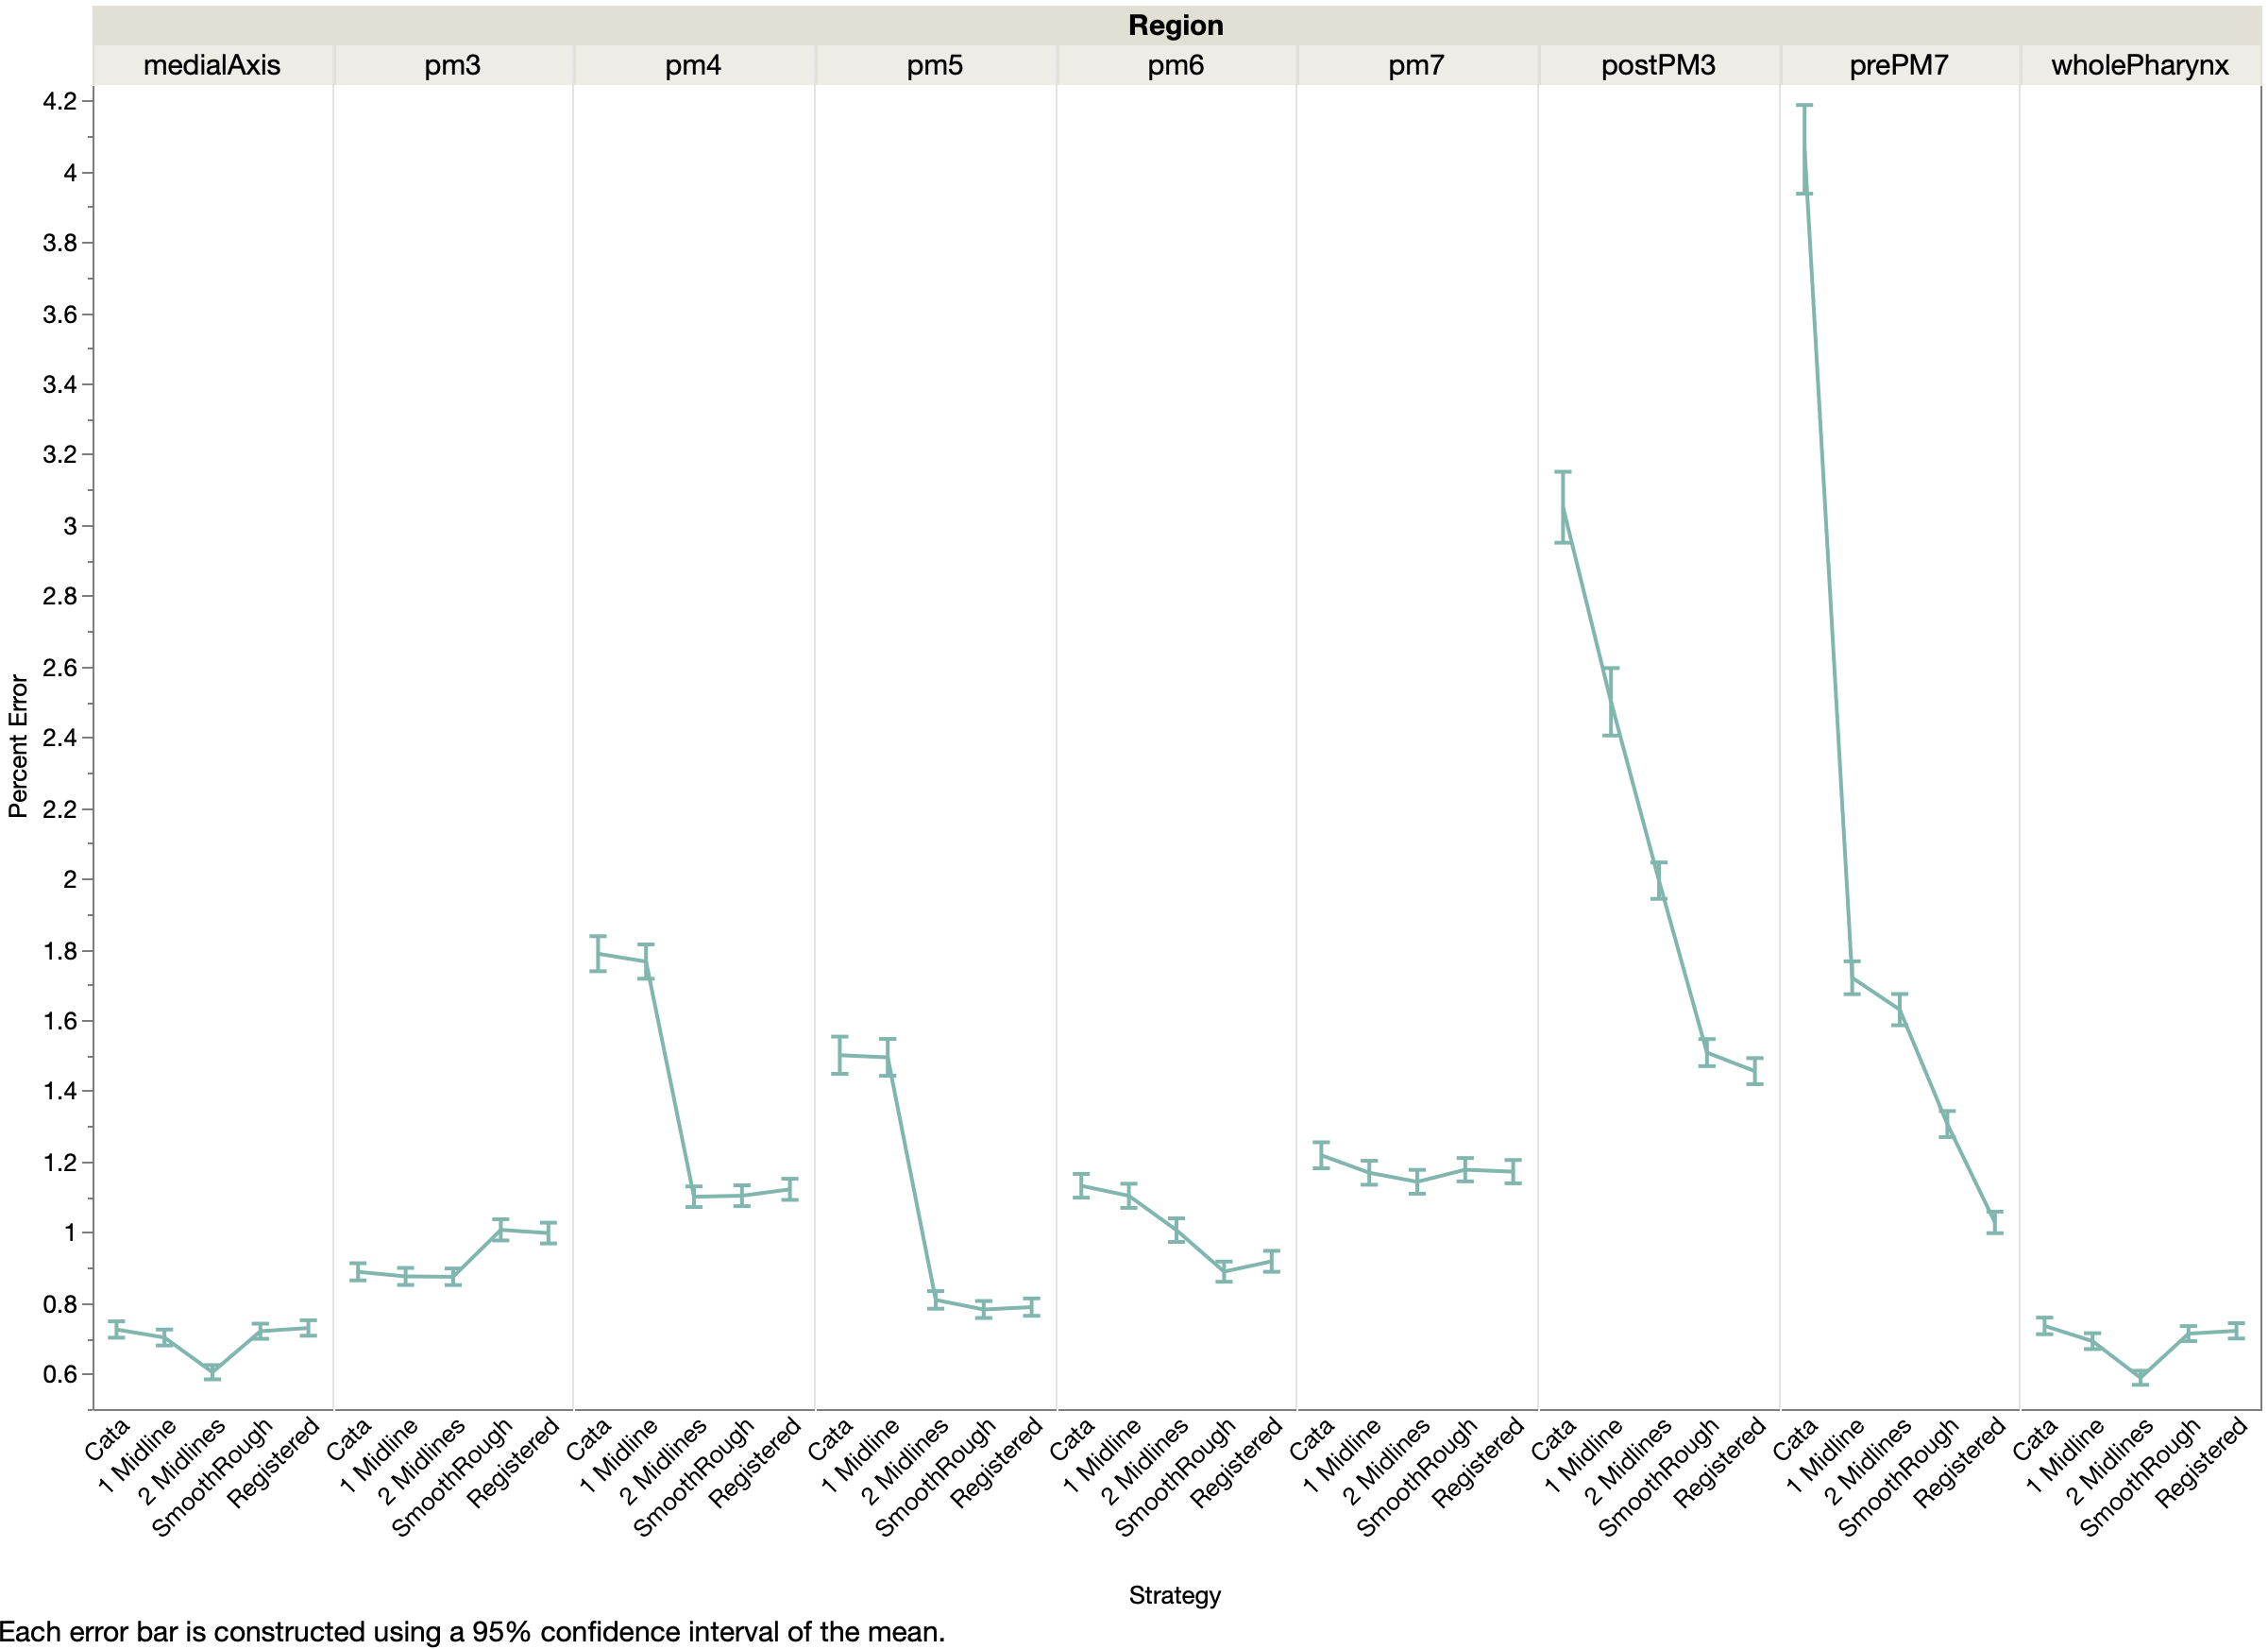
\includegraphics[scale=0.15]{Figures/rendered_files/error_by_strategy_synthetic}
%     \decoRule
%     \caption[Error by strategy in the synthetic data set]{}
%     \label{fig:PercentErrorSynthetic}
% \end{figure}